% Tugas 2 Kelompok 4
% Akbar Pambudi Utomo (1154094)
% Julham Ramadhana (1154069)
% Andi Wadi Afriandyka (1154113)
% Andi Nurfadillah Ali ()
% Hanna Theresia Siregar (1154009)
% Pebridayanti Hasibuan (1154118)


\section{Shapefile}
\subsection{Pengertian Shapefile}
Shapefile ArcView memiliki format data tersendiri yang disebut dengan shapefiles. 
Shapefiles adalah format data yang menyimpan lokasi geometrik dan informasi atribut dari suatu feature geografis. 
Pada umumnya kita hanya butuh satu file kerja seperti file Microsoft Worl dengan extension file *.doc, 
akan tetapi shapefile memiliki perbedaan, yaitu bahwa satu shapefile memiliki beberapa file yang saling berkaitan satu sama lainnya. 
Beberapa file ini memiliki extension yang 42 berbeda-beda yang disimpan dalam workspace yang sama.
Catatan : tiga file extension pertama adalah bagian file extension yang harus ada dalam sebuah shapefile, file extension berikutnya sifatnya optional.
Fitur geografis di shapefile dapat ditunjukkan oleh titik, garis, atau poligon (area). Ruang kerja yang berisi shapefile
mungkin juga berisi table dBase, yang dapat menyimpan atribut tambahan yang dapat digabungkan ke fitur shapefile.
Semua file yang memiliki ektensi seperti file .txt, .asc, .csv atau tab muncul di ArcCatalog sebagai file text secara default.
Akan tetapi, pada kotak dialog Opsi Kita dapat memilih tipe file mana yang harus direpresentasikan sebagai file
teks dan seharusnya tidak ditampilkan di pohon Catalog. Ketika file teks berisi nilai koma dan tab-delimited,
kita bisa melihat isi file di tampilan table ArcCatalog dan menggabungkannya ke dalam fitur geografis. file teks bisa juga kita hapus, tetapi isinya hanya bisa dibaca di ArcCatalog.\cite{kennedy2013introducing}
"Shapefile" adalah seperangkat file komputer yang digunakan untuk menyimpan informasi geografis (mis., Batas saluran sensus) 
dan tabel atribut yang terkait dengan informasi geografis (mis., Perumahan sensus dan karakteristik demografis). Shapefiles dapat 
dimanipulasi menggunakan sistem informasi geografis (SIG); ArcView 8.3 (ESRI, Redlands, CA) digunakan dalam proyek ini. 
Paket pajak shapefile diperoleh dari kantor penilai pajak Fulton dan Gwinnett County. Shapefile ini mengandung poligon yang sesuai 
dengan lokasi dan dimensi setiap paket tanah kena pajak di county. Alamat setiap paket disimpan dalam tabel atributnya.
Shapefile ESRI atau biasa disebut shapefila adalah format data geospasial yang umum untuk perangkat lunak sistem informasi geografis, dengan pengertian bahwa shape merupakan properti intrinsik utama untuk sistem visual manusia. manusia lebih sering mengasosialisasikan objek dengan bentuknya ketimbang elemen lainnya (warna misalnya), pada umumnya, citra yang dibentuk oleh mata merupakan citra dwimatra (2 dimensi), sedangkan objek yang dilihat umumnya berbentuk trimatra (3 dimensi). informasi bentuk objek dapat diekstansi dari citra pada permulaan pra-pengolahan dan segmentasi citra. salah satu tantangan utama pada komputer vision adalah merepresentasikan bentuk, atau aspek-aspek penting dari bentuk.

\subsection{Struktur Data Shapefile}
Geodatabase adalah struktur data yang kuat dan canggih. selain topologi yang anda dapatkan secara gratis, area dan sekeliling area yang
digambarkan dengan fitur linier. Namun, ESRI juga mendukung struktur data yang jauh lebih rumit: shapefile. sebuah shapefile dapat menggabungkan dua elemen penting yang dimiliki oleh geodatabase(komponen geografis dan database atribut) Perangkat lunak 
basis data adalah sistem manajemen basis data yang dinamai dBASE. Shapefile tertentu dibatasi hanya untuk mewakili satu dari jenis berikut: titik, multipoint, polyLines, atau poligon dengan titik. masing-masing titik memiliki catatan database relasional. Jika sejumlah titik dianggap objek yang sama, maka objek tersebut hanya memiliki satu record di tabel atribut. seperti pada geodatabases, polylines dapat disusun dari satu atau lebih jalur terhubung ataupun terputus-putus. Namun, jalur diperbolehkan untuk disusun hanya dari segmen garis lurus. Poligon dalam shapefile memiliki kemiripan dengan poligon basis geodata, namun tidak ada topologi yang ada dan tidak ada yang dapat diciptakan. setiap poligon berdiri sendiri. Hal ini digambarkan secara lengkap oleh satu entitas linier: urutan segmen yang dimulai di satu lokasi geografis dan kembali ke lokasi tersebut. mungkin ada poligon yang berdekatan atau tidak. poligon lain mungkin tumpang tindih. Lihat gambar berikut :
\begin{figure} [ht]
	\centerline{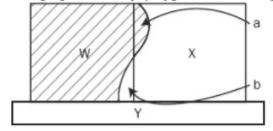
\includegraphics[width=1\textwidth]{figures/shapefilepoligon.JPG}}
	\caption{Gambar Shapefile Poligon}
	\label{shapefilepoligon}
	\end{figure}
Gambar silabus shapefile menggambarkan masalah dengan tumpang tindih dan kesenjangan. (Poligon W memiliki poligon batas kanan melengkung, X memiliki batas kiri lurus)\ref{shapefilepoligon}
Masalah dimana shapefiles sangat rentan adalah mungkin ada potongan tumpang tindih atau kekosongan-kekosongan (gap) antara poligon yang dimaksud, dan tidak ada yang dapat anda lakukan jika data tetap dalam format shapefile. Pada gambar diatas sliver 'a' diklaim oleh W dan X, sedangkan sliver 'b' tidak ada pada keduanya. Area geografis yang dipartisi enjadi poligon shapefile yang saling menggairahkan akan memiliki informasi duplikat. karena batas total masing-masing poligon didefinisikan untuk poligon itu, setiap garis umum adalah "digital ganda". Selanjutnya, ada dua batasan independen, dan anda tidak memiliki jaminan bahwa mereka kongruen. Dengan geodatabases, anda dapat membuat peraturan topologi untuk memastikan bahwa poligon tidak tumpang tindih atau memiliki celah, namun tidak dengan shapefile, anda tidak mendapatkan area dari perimeter sebagai atribut. keuntungan dari representasi shapefile adalah kesederhanaan, kecepatan pemrosesan, kecepatan menggambar, dan biasanya, ekonomi penyimpanan. shapefiles berguna bila anda tidak memerlukan geoprocessing yang canggih. Sadarilah bahwa banyak kumpulan data GIS telah dimasukkan ke dalam format shapefile. Mungkin ada banyak konversi ke format geodatabase di masa depan anda jika anda ingin menggunakan kumpulan data tersebut di geoprocessing.\cite{kennedy2013introducing}

\subsection{Daftar beberapa file extension}
\begin{enumerate}
    \item 1.shp - File yang menyimpan feature geometri (diperlukan dalam sebuah shapefile) 
    \item 2.shx - File yang menyimpan index dari feature geometri (diperlukan dalam sebuah shapefile) 
    \item 3.dbf - File dBASE yang menyimpan informasi atribut dari suatu feature (diperlukan dalam sebuah shapefile) 
    \item 4.sbn dan *.sbx – File yang menyimpan spatial index dari feature (optional) 
    \item 5.fbn dan *.fbx – File yang menyimpan spatial index dari feature shapefile yang read-only (optional) 
    \item 6.ain dan *.aih – File yang menyimpan index atribut dari field yang aktif dalam sebuah tabel (optional) 
    \item 7.prj - File yang menyimpan informasi koordinat dari sebuah shapefile, file ini dapat muncul jika kita menggunakan ArcView Projection Utility (optional).
\end{enumerate}
\subsubsection{Contoh penggunaan extension shapefile}
\begin{enumerate}
    \item 1. read.shapefile (form.name) 
    \item 2. read.shp (shp.name) 
    \item 3. read.shx (shx.name)
    \item 4. read.dbf (dbf.name, sundulan = FALSE)
    \item 5. write.shapefile (shapefile, out.name, arcgis = FALSE) 
    \item 6. write.shp (shp, out.name) 
    \item 7. write.shx (SHX, out.name)
    \item 8. write.dbf (DBF, out.name, arcgis = FALSE) 
    \item 9. calc.header (shapefile) 
    \item 10. add.xy (shapefile)
\end{enumerate}
\subsubsubsection{Bentuk file}
\begin{itemize}
    \item *.scaleXY (shapefile, scale.factor)
    \item *.convert.to.shapefile (shpTable, attTable, bidang, jenis) 
    \item *.convert.to.simple (shp)
    \item *.change.id (shpTable, newFieldAsVector) 
    \item *.dp (poin, toleransi)
\end{itemize}

\subsection{Contoh Script Shapefile}

## Not run: 

#Read entire shapefile 
shapefile <- read.shapefile("links") 

#Write entire shapefile 
write.shapefile(shapefile, "temp", T) 

#Read shp, shx, or dbf file 
dbf <- read.dbf("links.dbf") 

#Write shp, shx, or dbf file 
write.dbf(dbf, "links.dbf", T) 

#Calculate header (to clean up GeoMedia shapefile exports) 
shapefile <- calc.header(shapefile) 

#Add the X and Y coordinates to the dbf list of the shapefile list object 
shapefile <- add.xy(shapefile)

#Scale the shapefile by scale.factor 
shapefile <- scaleXY(shapefile, scale.factor) 

#Samples of using the convert.to.shapefile function to write out simple shapefiles 
#from basic R data.frames 

#Point 
dd <- data.frame(Id=c(1,2),X=c(3,5),Y=c(9,6)) 
ddTable <- data.frame(Id=c(1,2),Name=c("Item1","Item2")) 
ddShapefile <- convert.to.shapefile(dd, ddTable, "Id", 1) 
write.shapefile(ddShapefile, "c:/test", arcgis=T) 

#PolyLine 
dd <- data.frame(Id=c(1,1,1,2,2,2),X=c(3,5,8,6,7,8),Y=c(9,8,3,6,7,4)) 
ddTable <- data.frame(Id=c(1,2),Name=c("Item1","Item2")) 
ddShapefile <- convert.to.shapefile(dd, ddTable, "Id", 3) 
write.shapefile(ddShapefile, "c:/test", arcgis=T) 

#Polygon 
dd <- data.frame(Id=c(1,1,1,1,2,2,2,2),X=c(3,5,8,3,6,7,8,6),Y=c(9,8,3,9,6,7,4,6)) 
ddTable <- data.frame(Id=c(1,2),Name=c("Item1","Item2")) 
ddShapefile <- convert.to.shapefile(dd, ddTable, "Id", 5) 
write.shapefile(ddShapefile, "c:/test", arcgis=T)

#Convert to list of shapes 
ddAsList <- by(dd,dd$Id, function(x) x) 

#Convert to data.frame 
dd <- do.call(rbind, ddAsList) 

#Read in shp file and convert to simple format 
shpTest <- read.shp("c:/test.shp") 
simpleShpFormat <- convert.to.simple(shpTest) 
simpleShpFormat <- change.id(simpleShpFormat, c("a","b")) 
simpleAsList <- by(simpleShpFormat, simpleShpFormat[,1], function(x) x) 
backToShape <- convert.to.shapefile(simpleShpFormat, 
data.frame(index=c("a","b")), "index", 5) 
write.shapefile(backToShape, "c:/test", arcgis=T) 

#Polyline simplification with dp algorithm 
x <- c(5,3,4,1,8,9,10,11)
 y <- c(6,4,2,1,1,5,2,3) 
points <- list(x=x,y=y) 
plot(points, type="l") 
simpleLine <- dp(points, 2) 
lines(simpleLine, type="l", col="blue") 

## End(Not run)

\subsection{Komponen Teknis}
Komponen yang ada pada sebuah aplikasi GIS
mempunyai fungsi utama untuk membaca dan menulis
data spasial, baik yang tersimpan dalam sebuah
shapefile (*.shp) atau tersimpan ke dalam sebuah
database (Eddy 2006).
Dalam MapServer yang sudah berjalan ada beberapa
Komponen utama yang digunakan secara peneuh untuk
menjalankan Aplikasi GIS untuk menangani data
spasial baik yang tersimpan dalam sebuah flat file atau
juga dalam DBMS yaitu :
1. SHAPELIB
Shapelib merupakan library yang ditulis
menggunakan bahasa pemrograman C yang
digunakan untuk melakukan proses read terhadap
Shapefile (*.shp) yang sudah didefinisikan ESRI
(Environmental System Research Institute).
Format dalam shapefile umum digunakan untuk
menyimpan data vector simple (tanpa topologi)
dengan atribut, shapefile merupakan format data
default yang digunakan dalam GIS.

\subsection{Deskripsi Teknis Shapefile}
SDE, ARC / INFO, PC ARC / INFO, Data Otomasi Kit (DAK ™ ), dan ArcCAD ® 
Perangkat lunak menyediakan penerjemah data form-to-coverage, dan ARC / INFO juga menyediakan a 
penerjemah coverage-to-shape. Untuk pertukaran dengan format data lainnya, shapefile 
spesifikasi diterbitkan dalam makalah ini. Aliran data lainnya, seperti yang berasal dari global 
receiver positioning system (GPS), juga dapat disimpan sebagai shapefile atau X, Y event tables. 

\subsection{Mengapa Harus menggunakan Shapefile}
Sebuah shapefile menyimpan geometri nontopologis dan informasi atribut untuk ruang 
fitur dalam kumpulan data Geometri untuk fitur disimpan sebagai bentuk yang terdiri dari satu set 
koordinat vektor 
Karena shapefile tidak memiliki overhead pengolahan dari struktur data topologi, 
mereka memiliki kelebihan dibandingkan sumber data lain seperti kecepatan dan edit gambar yang lebih cepat 
kemampuan. Shapefiles menangani fitur tunggal yang tumpang tindih atau tidak bersebelahan. Mereka 
Juga biasanya membutuhkan lebih sedikit ruang disk dan lebih mudah dibaca dan ditulis. 
Shapefiles dapat mendukung fitur titik, garis, dan area. Fitur area direpresentasikan sebagai 
loop tertutup, poligon digital ganda. Atribut disimpan dalam file format dBASE ® . 
Setiap record atribut memiliki hubungan satu lawan satu dengan catatan bentuk yang terkait

\subsection{Shapefile dapat dibuat dengan 4 Metode Umum}
Ekspor Shapefiles dapat dibuat dengan mengekspor sumber data ke shapefile
ARC / INFO® , PC ARC / INFO®, Spasial Database Engine ™ (SDE ™ ), ArcView® GIS,
atau perangkat lunak Business MAP ™ .
Digitize Shapefiles dapat dibuat secara langsung dengan mendigitalkan bentuk menggunakan ArcView GIS
alat pembuatan fitur
Pemrograman Menggunakan Avenue ™ (ArcView GIS), MapObjects ™ , ARC Macro
Bahasa (AML ™ ) (ARC / INFO), atau Simple Macro Language (SML ™ )
(PC ARC / INFO) perangkat lunak, Anda dapat membuat shapefile dalam program Anda.
Menulis langsung ke spesifikasi shapefile dengan membuat sebuah program. 
